\documentclass[mathNotesPreamble]{subfiles}
\begin{document}
%\relscale{1.4} %TODO
\section{15.3: Partial Derivatives}

  Recall that for functions with one independent variable, say $y=f(x)$, the derivative measures the change in $y$ with respect to $x$. For functions with multiple independent variables, we compute derivatives with respect to each variable.

  \begin{center}
    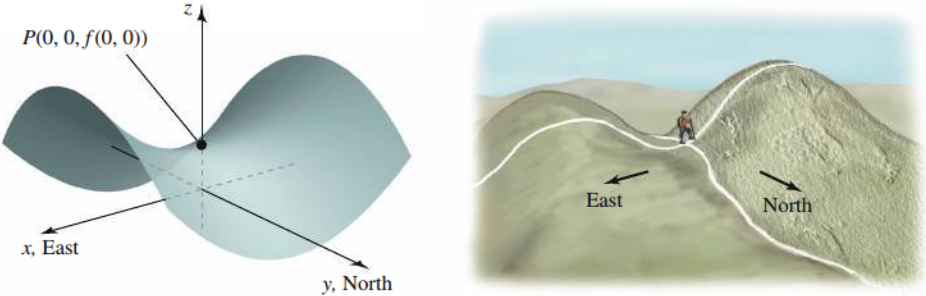
\includegraphics[width=0.45\linewidth]{images/briggs_15_03/fig15_30}
  \end{center}

  \begin{defn*}[Partial Derivatives]
    The \textbf{partial derivative of $f$ with respect to $x$ at the point $(a,b)$ is}
      \[f_x(a,b)=\lim_{h\to 0} \frac{f(a+h,b)-f(a,b)}{h}.\]
    The \textbf{partial derivative of $f$ with respect to $y$ at the point $(a,b)$ is}
      \[f_y(a,b)=\lim_{h\to 0} \frac{f(a,b+h)-f(a,b)}{h},\]
    provided these limits exist.
  \end{defn*}

  \begin{center}
    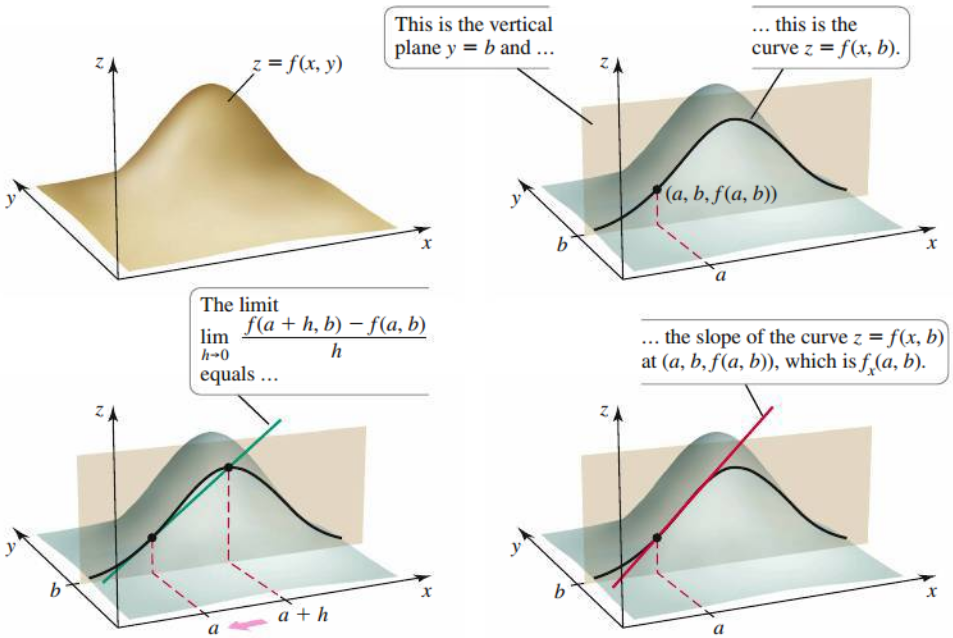
\includegraphics[width=0.5\linewidth]{images/briggs_15_03/fig15_31}
  \end{center}
  \pagebreak

  When evaluating a partial derivative at a point $(a,b)$, we denote this
    \[\frac{\partial f}{\partial x}(a,b)=\left.\frac{\partial f}{\partial x}\right|_{(a,b)}=f_x(a,b) \textnormal{ and }\frac{\partial f}{\partial y}(a,b)=\left.\frac{\partial f}{\partial y}\right|_{(a,b)}=f_y(a,b)\]
  \begin{ex*}
    For the following functions, find the first partial derivatives. If a point is provided, evaluate the partial derivatives.
  \end{ex*}
  \begin{tasks}[after-item-skip=\stretch{1}, label=](1)
    \task $f(x,y)=x^8+3y^9+8$
    \task $g(x,y)=6x^5y^2+2x^3y+5$
  \end{tasks}
  \vspace*{\stretch{1}}
  \pagebreak

  \begin{tasks}[after-item-skip=\stretch{1}, label=](1)
    \task $h(s,t)=\dfrac{s-t}{4s+t}$ at $(s,t)=(2,-3)$
    \task $k(x,y)=\tan\inv\!\parens{3x^2y^2}$ at $(x,y)=(1,1)$
    \task $\ell(w,v)=\ds\int_v^w g(u)\,du$
  \end{tasks}
  \vspace*{\stretch{1}}
  \pagebreak

  \textbf{Higher-Order Partial Derivatives:}

  \begin{center}
    \renewcommand{\arraystretch}{2.25}
    \begin{tabular}{@{}r@{$\ =\ $}lM{0.2\linewidth}l@{}}
      \toprule
      $\dfrac{\partial}{\partial x}\parens{\dfrac{\partial f}{\partial x}}$&$ \dfrac{\partial^2 f}{\partial x^2}$&
      $\parens{f_x}_x=f_{xx}$&
      ``$d$ squared $f\ dx$ squared or $f-x-x$''\\
      %
      $\dfrac{\partial}{\partial y}\parens{\dfrac{\partial f}{\partial y}}$&$ \dfrac{\partial^2 f}{\partial y^2}$&
      $\parens{f_y}_y=f_{yy}$&
      ``$d$ squared $f\ dy$ squared or $f-y-y$''\\
      %
      $\dfrac{\partial}{\partial x}\parens{\dfrac{\partial f}{\partial y}}$&$ \dfrac{\partial^2 f}{\partial x \partial y}$&
      $\parens{f_y}_x=f_{yx}$&
      ``$f-y-x$''\\
      %
      $\dfrac{\partial}{\partial y}\parens{\dfrac{\partial f}{\partial x}}$&$ \dfrac{\partial^2 f}{\partial y \partial x}$&
      $\parens{f_x}_y=f_{xy}$&
      ``$f-x-y$''\\\bottomrule
    \end{tabular}
  \end{center}

  \noindent
  The order of differentiation is important when finding \textbf{mixed partial derivatives} $f_{xy}$ and $f_{yx}$.
  \begin{ex*}
    Find the four 2nd-order partial derivatives of the following functions
  \end{ex*}
  \begin{tasks}[after-item-skip=\stretch{1}, label=](1)
    \task $z=4ye^{3x}$
    \task $f(x,y)=\sin^2(x^3y)$
  \end{tasks}
  \vspace*{\stretch{1}}
  \pagebreak

  \begin{thmBox*}[Theorem 15.4: (Clairut) Equality of Mixed Partial Derivatives]
    Assume $f$ is defined on an open set $D$ of $\bbr^2$, and that $f_{xy}$ and $f_{yx}$ are continuous throughout $D$. Then $f_{xy}=f_{yx}$ at all points of $D$.
  \end{thmBox*}

  \vspace*{0.5\baselineskip}\noindent
  \textit{Note:} Clairut's theorem also extends to higher order derivatives of $f$.

  \begin{ex*}
    \textbf{Ideal Gas Law:} The pressure $P$, volume $V$, and temperature $T$ of an ideal gas are related by the equation $PV=kT$, where $k>0$ is a constant depending on the amount of gas.
  \end{ex*}
  \begin{tasks}[after-item-skip=\stretch{1}, label=](1)
    \task Determine the rate of change of the pressure with respect to the volume
    \task Determine the rate of change of the pressure with respect to the temperature
  \end{tasks}
  \vspace*{\stretch{1}}
  \pagebreak

  \begin{defn*}[Differentiability]
    The function $z=f(x,y)$ is \textbf{differentiable at $(a,b)$} provided $f_x(a,b)$ and $f_y(a,b)$ exist and the change $\Delta z=f(a+\Delta x, b+\Delta y)-f(a,b)$ equals
      \[\Delta z=f_x(a,b)\Delta x+ f_y(a,b)\Delta y=\eps_1\Delta x+\eps_2\Delta y,\]
    where for fixed $a$ and $b$, $\eps_1$ and $\eps_2$ are functions that depend only on $\Delta x$ and $\delta y$, with $\parens{\eps_1,\eps_2}\to (0,0)$ as $\parens{\Delta x,\Delta y}\to(0,0)$. A function is \textbf{differentiable} on an open set $R$ if it is differentiable at every point of $R$.
  \end{defn*}
  \vspace*{\stretch{1}}

  \begin{thmBox*}[Theorem 15.5: Conditions for Differentiability]
    Suppose the function $f$ has partial derivatives $f_x$ and $f_y$ defined on an open set containing $(a,b)$, with $f_x$ and $f_y$ continuous at $(a,b)$. Then $f$ is differentiable at $(a,b)$.
  \end{thmBox*}
  \vspace*{\stretch{1}}

  \begin{thmBox*}[Theorem 15.6: Differentiable Implies Continuous]
    If a function $f$ is differentiable at $(a,b)$, then it is continuous at $(a,b)$.
  \end{thmBox*}
  \begin{ex*}
    Why is the function
      \[f(x,y)=\begin{cases}
        \frac{3xy}{x^2+y^2},& \textnormal{if } (x,y)\neq (0,0)\\
        0,& \textnormal{if } (x,y)=(0,0)
      \end{cases}\]
    not continuous at $(x,y)=(0,0)$?
  \end{ex*}
  \vspace*{\stretch{10}}
  \pagebreak
  
\end{document}